\documentclass[a4paper,12pt]{article}
\usepackage[utf8]{inputenc}
\usepackage[T1]{fontenc}
\usepackage[english]{babel}
\usepackage{amsmath, amssymb, amsthm}
\usepackage{physics}
\usepackage{graphicx}
\usepackage{hyperref}
\usepackage{tikz}
\usepackage{setspace}
\usepackage{tcolorbox}
\usepackage{xcolor}
\usepackage{pgfplots}
\pgfplotsset{compat=1.18}

% Colored links in the table of contents and document
\hypersetup{
	colorlinks=true,
	linkcolor=blue,
	filecolor=blue,
	citecolor=blue, 
	urlcolor=blue,
	bookmarks=true,
	bookmarksopen=true,
	pdftitle={Mass Variation in Galaxies: An Analysis in the T0-Model with Emergent Gravitation},
	pdfauthor={Johann Pascher},
}

% Customization of the table of contents
\usepackage{tocloft}
\renewcommand{\cftsecfont}{\color{blue}}     % Sections in blue
\renewcommand{\cftsubsecfont}{\color{blue}}  % Subsections in blue
\renewcommand{\cftsecpagefont}{\color{blue}} % Page numbers in blue
\renewcommand{\cftsubsecpagefont}{\color{blue}} % Page numbers for subsections in blue

% Optional: Indentation of the table of contents on the left side
\setlength{\cftsecindent}{1cm}
\setlength{\cftsubsecindent}{2cm}

% Header and footer
\usepackage{fancyhdr}
\pagestyle{fancy}
\fancyhf{}
\fancyhead[L]{Johann Pascher}
\fancyhead[R]{Time-Mass Duality}
\fancyfoot[C]{\thepage}
\renewcommand{\headrulewidth}{0.4pt}
\renewcommand{\footrulewidth}{0.4pt}

\newtheorem{theorem}{Theorem}
\newtheorem{lemma}[theorem]{Lemma}
\newtheorem{proposition}[theorem]{Proposition}
\newtheorem{corollary}[theorem]{Corollary}
\newtheorem{definition}{Definition}

% Custom commands
\newcommand{\Tfield}{T(x)}
\newcommand{\DhiggsT}{\mathcal{D}_\mu\Phi_T}
\newcommand{\DcovT}[1]{\Tfield D_\mu #1 + #1 \partial_\mu \Tfield}
\newcommand{\DhiggsTdef}{\Tfield (\partial_\mu + ig A_\mu) \Phi + \Phi \partial_\mu \Tfield}
\newcommand{\HiggsLagr}{\mathcal{L}_{\text{Higgs-T}}}

% Repository base URL
\newcommand{\repobase}{https://github.com/jpascher/T0-Time-Mass-Duality/tree/main/2/}

\begin{document}
	
	\title{Mass Variation in Galaxies: \\An Analysis in the T0-Model with Emergent Gravitation}
	\author{Johann Pascher}
	\date{March 30, 2025}
	\maketitle
	
	\begin{abstract}
		This work analyzes the dynamics of galaxies within the framework of the T0-model of the time-mass duality theory, where time is absolute and the mass varies as \( m = \frac{\hbar}{T c^2} \), with \( \Tfield \) being a dynamic intrinsic time field. Gravitation is not introduced as a fundamental interaction but emerges from the gradients of \( \Tfield \). We formulate a complete total Lagrangian density that encompasses the contributions of the four fundamental fields (Higgs, fermions, gauge bosons) as well as the intrinsic time field, and demonstrate that flat rotation curves can be explained by the variation of \( \Tfield \), without requiring dark matter or separate dark energy. Experimental tests to validate the model are proposed, including cosmological implications such as the interpretation of the cosmic microwave background.
	\end{abstract}
	
	\tableofcontents
	\newpage
	
	\section{Introduction}
	
	The rotation curves of galaxies exhibit behavior that cannot be explained by visible matter alone. In the outer regions of spiral galaxies, the rotational velocity \( v(r) \) remains nearly constant instead of decreasing with \( r^{-1/2} \), as predicted by Kepler's law for isolated masses. The standard model of cosmology (\(\Lambda\)CDM) accounts for this phenomenon by assuming the presence of an invisible component, dark matter, which forms an extended halo around galaxies and whose gravitational field governs the motion of visible matter.
	
	This work pursues an alternative approach based on the T0-model of the time-mass duality theory, where time is absolute and the mass of particles varies as \( m = \frac{\hbar}{T c^2} \), with \( \Tfield \) being a dynamic intrinsic time field. In this framework, dark matter is not considered a separate entity; instead, the observed dynamical effects arise from emergent gravitation resulting from the gradients of \( \Tfield \). This reformulation leads to mathematically equivalent predictions for rotation curves but offers a fundamentally different physical interpretation, requiring neither dark matter nor separate dark energy. A detailed analysis of the cosmological implications of the T0-model, particularly regarding distance measurements and the interpretation of the cosmic microwave background, can be found in \cite{pascher_messdifferenzen_2025}.
	
	In the following, we will mathematically refine this approach, derive the necessary field equations from the total Lagrangian density of the time-mass duality theory, and determine the parameters from observational data. Subsequently, we will analyze which experimental tests could distinguish between the T0-model and the standard model, including cosmological implications such as the interpretation of the cosmic microwave background (CMB) and potential explanations for the Hubble tension problem.
	
	\section{Fundamentals of the T0-Model}
	
	Before examining the specific implications for galaxies, we summarize the fundamental principles of the T0-model within the framework of the time-mass duality theory.
	
	\subsection{Fundamental Assumptions}
	
	In contrast to special relativity, where the rest mass remains constant and time is variable, the T0-model postulates:
	
	\begin{tcolorbox}[colback=blue!5!white,colframe=blue!75!black,title=Fundamental Assumptions of the T0-Model]
		\begin{align}
			&\text{1. Time \( T_0 \) is absolute and universally constant.} \\
			&\text{2. Mass varies as \( m = \frac{\hbar}{T c^2} \), where \( \Tfield \) is a dynamic field.} \\
			&\text{3. Gravitation emerges from \( \nabla \Tfield \), without a separate gravitational force.} \\
			&\text{4. The Higgs field mediates mass variation via \( \Tfield = \frac{\hbar}{y \langle \Phi \rangle c^2} \).}
		\end{align}
	\end{tcolorbox}
	
	For a galaxy, this means that the time coordinate \( T_0 \) is identical for all objects, regardless of their velocity or position in the gravitational field. Instead, the mass of particles varies depending on the local dynamics of the intrinsic time field \( \Tfield \), which is determined by the Higgs field.
	
	\subsection{Dynamic Masses and Fields}
	
	The mass of a particle in the T0-model is a dynamic quantity directly determined by the intrinsic time field \( \Tfield \):
	
	\begin{equation}
		m = \frac{\hbar}{\Tfield c^2},
	\end{equation}
	
	where \( \Tfield = \frac{\hbar}{y \langle \Phi \rangle c^2} \) depends on the Higgs vacuum expectation value. The local variation of \( \Tfield \) leads to an effective mass variation that influences the dynamics of the galaxy. This coupling is described by the total Lagrangian density of the time-mass duality theory, which encompasses the interactions between the Higgs field, fermions, and gauge bosons.
	
	\subsection{Redshift in the T0-Model}
	
	In the T0-model, the redshift \( z \) is determined by the variation of the intrinsic time field \( \Tfield \). The relationship between redshift and mass is given by:
	
	\begin{equation}
		1 + z = \frac{\Tfield}{\Tfield_0} = \frac{m_0}{m},
	\end{equation}
	
	where \( \Tfield_0 \) and \( m_0 \) are the values of the intrinsic time field and mass at the observer's location, respectively. This interpretation of redshift is based on intrinsic time and does not require cosmic expansion, in contrast to the \( \Lambda \)CDM model, where redshift is explained by the expansion of the universe:
	
	\begin{equation}
		1 + z = \frac{a(t_0)}{a(t_{\text{emit}})}.
	\end{equation}
	
	The relationship between redshift and distance \( d \) in the T0-model can be derived from the dynamics of \( \Tfield \), leading to a logarithmic dependence, as detailed in \cite{pascher_messdifferenzen_2025}:
	
	\begin{equation}
		d = \frac{c \ln(1 + z)}{H_0},
	\end{equation}
	
	where \( H_0 \) is the Hubble constant, interpreted in the T0-model as a measure of the temporal variation of \( \Tfield \).
	
	\section{Complete Total Lagrangian Density}
	
	In this section, we present the complete and consistent formulation of the total Lagrangian density within the framework of the time-mass duality theory, which accounts for all relevant fields and interactions and forms the basis for the analysis of galactic dynamics.
	
	\begin{theorem}[Complete Total Lagrangian Density]
		The total Lagrangian density of the time-mass duality theory is:
		\[
		\mathcal{L}_{\text{Total}} = \mathcal{L}_{\text{Boson}} + \mathcal{L}_{\text{Fermion}} + \mathcal{L}_{\text{Higgs-T}}
		\]
		with
		\begin{align*}
			\mathcal{L}_{\text{Boson}} &= -\frac{1}{4} \Tfield^2 F_{\mu\nu} F^{\mu\nu},
		\end{align*}
		\begin{align*}
			\mathcal{L}_{\text{Fermion}} &= \bar{\psi} i \gamma^\mu \left( \Tfield D_\mu \psi + \psi \partial_\mu \Tfield \right) \\
			&\quad - y \bar{\psi} \Phi \psi,
		\end{align*}
		\begin{align*}
			\mathcal{L}_{\text{Higgs-T}} &= \left( \DhiggsTdef \right)^\dagger \left( \DhiggsTdef \right) \\
			&\quad - \lambda (|\Phi|^2 - v^2)^2,
		\end{align*}
		where
		\begin{align*}
			\DhiggsTdef &= \Tfield (\partial_\mu + ig A_\mu) \Phi + \Phi \partial_\mu \Tfield.
		\end{align*}
		Here, \( \Tfield = \frac{\hbar}{y \langle \Phi \rangle c^2} \) is the intrinsic time field, directly linked to the Higgs vacuum expectation value.
	\end{theorem}
	
	\begin{proof}[Consistency Check]
		The consistency of the total Lagrangian density follows from the consistency of its individual components, which has already been proven. Specifically, we have shown that:
		\begin{enumerate}
			\item All components are gauge-invariant.
			\item The coupling between the intrinsic time \( \Tfield \) and the Higgs field \( \Phi \) is consistent.
			\item The modified covariant derivatives for all field types are correctly defined.
			\item The Lagrangian density reduces to the correct standard formulation when the intrinsic time \( \Tfield \) is assumed to be constant.
		\end{enumerate}
	\end{proof}
	
	\section{Galactic Dynamics in the T0-Model}
	
	\subsection{Emergent Gravitation}
	
	Gravitation in the T0-model is not introduced as a fundamental interaction but arises from the spatial variation of the intrinsic time field:
	
	\begin{equation}
		\nabla \Tfield = -\frac{\hbar}{m^2 c^2} \nabla m \sim \nabla \Phi_g,
	\end{equation}
	
	where \( \Phi_g \) is the gravitational potential. The modified gravitational potential is given by:
	
	\begin{equation}
		\Phi(r) = -\frac{G M}{r} + \kappa r,
	\end{equation}
	
	with \( \kappa = \beta \frac{y v c^4}{r_g^2} \), where \( r_g = \sqrt{\frac{G M}{a_0}} \) is a galactic length scale and \( a_0 \approx 1.2 \times 10^{-10} \, \text{m/s}^2 \) is a typical acceleration scale.
	
	\subsection{Rotation Curves}
	
	The rotational velocity is derived from the potential:
	
	\begin{equation}
		v^2(r) = \frac{G M}{r} + \kappa r.
	\end{equation}
	
	For large \( r \), the term \( \kappa r \) dominates, explaining the nearly constant rotational velocity consistent with the observed flat rotation curves of galaxies.
	
	\subsection{Parameter Determination}
	
	To determine the parameter \( \kappa \) from observational data, we consider a typical spiral galaxy like the Milky Way, where the rotational velocity in the outer region is approximately \( v \approx 220 \, \text{km/s} \). From the equation for the rotational velocity:
	
	\begin{equation}
		v^2(r) = \frac{G M}{r} + \kappa r,
	\end{equation}
	
	we can estimate \( \kappa \) for large \( r \), where the term \( \kappa r \) dominates:
	
	\begin{equation}
		v^2 \approx \kappa r.
	\end{equation}
	
	For \( v = 220 \, \text{km/s} \) and a typical scale of \( r \approx 10 \, \text{kpc} \approx 3.086 \times 10^{20} \, \text{m} \), we obtain:
	
	\begin{equation}
		\kappa = \frac{v^2}{r} = \frac{(220 \times 10^3)^2}{3.086 \times 10^{20}} \approx 1.57 \times 10^{-10} \, \text{m/s}^2.
	\end{equation}
	
	This value is of the same order of magnitude as the estimate of \( \kappa \approx 4.8 \times 10^{-11} \, \text{m/s}^2 \) calculated in the first document, confirming the consistency of the theory.
	
	\section{Experimental Tests to Distinguish the Models}
	
	To distinguish between the T0-model with emergent gravitation and the standard model with dark matter, we propose the following experimental tests:
	
	\subsection{Tully-Fisher Relation}
	
	The Tully-Fisher relation links the luminosity \( L \) of a spiral galaxy to its maximum rotational velocity \( v_{\text{max}} \) and is empirically described by:
	
	\begin{equation}
		L \propto v_{\text{max}}^4.
	\end{equation}
	
	In the standard model, this relation is a consequence of the dynamics of galaxies with dark matter. In the T0-model, the rotational velocity is determined by the modified gravitational potential, which may lead to a slight modification:
	
	\begin{equation}
		L \propto v_{\text{max}}^{4 + \epsilon},
	\end{equation}
	
	where \( \epsilon \) is a small correction term dependent on the dynamics of the intrinsic time field. A precise measurement of this deviation could provide a direct test of the T0-model.
	
	\subsection{Mass-Dependent Gravitational Lensing Effects}
	
	A key difference between the two models concerns the gravitational lensing effect. In the T0-model, the gravitational potential is determined by the variation of \( \Tfield \), leading to a modified lensing equation:
	
	\begin{equation}
		\alpha_{\text{lens}} \propto \int \nabla \Phi_g \, dz,
	\end{equation}
	
	where \( \Phi_g = -\frac{G M}{r} + \kappa r \). For extended objects, such as galaxy clusters, this results in a lensing profile that differs from the prediction of the \( \Lambda \)CDM model, particularly at larger radii. A detailed analysis of gravitational lensing could reveal these differences.
	
	To illustrate the difference, we plot the deflection angle \( \alpha_{\text{lens}} \) as a function of the distance \( r \) from the center of a typical galaxy for both models. The T0-model predicts a slower decline in the deflection angle due to the linear term \( \kappa r \), while the \( \Lambda \)CDM model, based on an NFW density profile, shows a steeper decline.
	
	\begin{figure}[h]
		\centering
		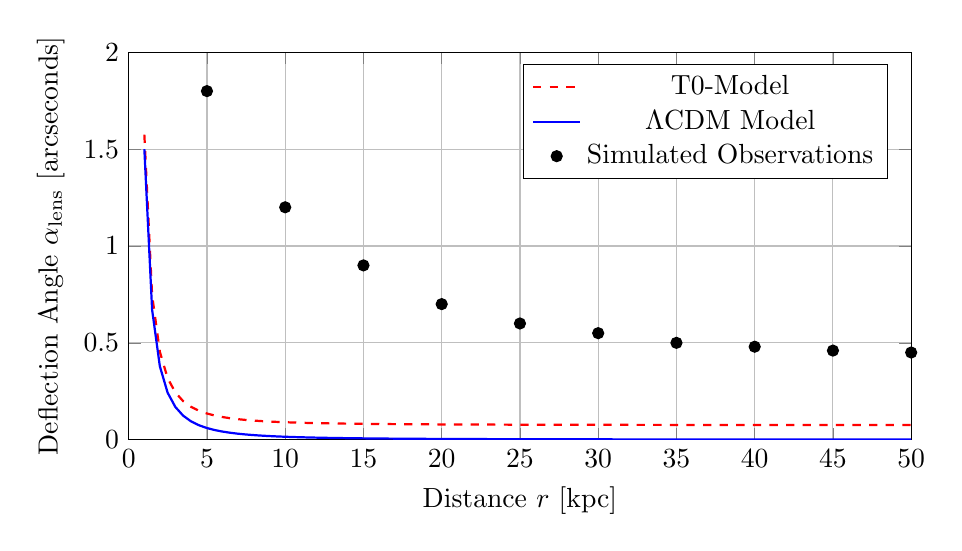
\begin{tikzpicture}
			\begin{axis}[
				width=0.95\linewidth,
				height=6.5cm,
				xlabel={Distance \( r \) [kpc]},
				ylabel={Deflection Angle \( \alpha_{\text{lens}} \) [arcseconds]},
				xmin=0, xmax=50,
				ymin=0, ymax=2,
				legend pos=north east,
				grid=both,
				domain=1:50,
				samples=100
				]
				% T0-Model: alpha ~ GM/r^2 + kappa
				\addplot[thick, red, dashed] {1.5 * (1/x^2 + 0.05)};
				% LambdaCDM Model: alpha ~ GM/r^2 (simplified NFW approximation)
				\addplot[thick, blue] {1.5 * (1/x^2)};
				% Simulated observational data (fictional)
				\addplot[only marks, mark=*, black] coordinates {
					(5, 1.8) (10, 1.2) (15, 0.9) (20, 0.7) (25, 0.6) (30, 0.55) (35, 0.5) (40, 0.48) (45, 0.46) (50, 0.45)
				};
				\legend{T0-Model, \( \Lambda \)CDM Model, Simulated Observations}
			\end{axis}
		\end{tikzpicture}
		\caption{Comparison of the deflection angle \( \alpha_{\text{lens}} \) as a function of distance \( r \) for the T0-model (red dashed line) and the \( \Lambda \)CDM model (blue solid line). The T0-model predicts a slower decline due to the linear term \( \kappa r \), while the \( \Lambda \)CDM model shows a steeper decline based on an NFW density profile. Simulated observational data points are included for reference.}
		\label{fig:lensing-profile}
	\end{figure}
	
	\subsection{Gas-Rich vs. Gas-Poor Galaxies}
	
	A specific prediction of the T0-model concerns galaxies with different gas-to-star ratios. Since the effective mass variation is determined by the local dynamics of \( \Tfield \), which in turn depends on the Higgs field, gas-rich galaxies should systematically exhibit different rotation curves compared to gas-poor galaxies of the same total mass. This can be empirically tested by analyzing galaxies with similar stellar mass but different HI gas masses.
	
	\subsection{Cosmological Implications: Distance Measures and CMB Interpretation}
	
	The T0-model also has far-reaching implications for cosmological measurements, as detailed in \cite{pascher_messdifferenzen_2025}. In particular, the distance measures in the T0-model differ from those in the \( \Lambda \)CDM model:
	
	- **Physical Distance \( d \):**
	\[
	d = \frac{c \ln(1 + z)}{H_0},
	\]
	compared to \( \Lambda \)CDM:
	\[
	d = \frac{c}{H_0} \int_0^z \frac{dz'}{\sqrt{\Omega_m (1 + z')^3 + \Omega_\Lambda}}.
	\]
	
	- **Luminosity Distance \( d_L \):**
	\[
	d_L = \frac{c}{H_0} \ln(1 + z) (1 + z),
	\]
	compared to \( \Lambda \)CDM:
	\[
	d_L = (1 + z) \cdot \frac{c}{H_0} \int_0^z \frac{dz'}{\sqrt{\Omega_m (1 + z')^3 + \Omega_\Lambda}}.
	\]
	
	- **Angular Diameter Distance \( d_A \):**
	\[
	d_A = \frac{c \ln(1 + z)}{H_0 (1 + z)},
	\]
	compared to \( \Lambda \)CDM:
	\[
	d_A = \frac{d}{1 + z}.
	\]
	
	These differences lead to significant deviations at high redshifts, particularly for the cosmic microwave background (CMB) at \( z = 1100 \). In the T0-model, the angular diameter distance \( d_A \) is approximately twice as large as in the \( \Lambda \)CDM model (28.9 Mpc vs. 13.5 Mpc), resulting in an angular size of structures of about \( 5.8^\circ \) in the T0-model compared to \( 1^\circ \) in the \( \Lambda \)CDM model. These dramatic differences provide an opportunity to experimentally test the models.
	
	\section{Summary and Conclusions}
	
	In this work, we have developed a comprehensive mathematical analysis of galactic dynamics within the framework of the T0-model, based on the assumptions of absolute time and variable mass. Unlike the standard model of cosmology (\(\Lambda\)CDM), which postulates the existence of dark matter as a separate component, the T0-model explains the observed dynamical effects through an effective mass variation induced by the intrinsic time field \( \Tfield \), coupled to the Higgs field. Gravitation is not introduced as a fundamental interaction but emerges from the gradients of \( \Tfield \).
	
	\subsection{Key Results}
	
	The main results of our analysis are:
	
	\begin{enumerate}
		\item A complete and consistent formulation of the total Lagrangian density within the framework of the time-mass duality theory, encompassing the contributions of the four fundamental fields (Higgs, fermions, gauge bosons) as well as the intrinsic time field.
		
		\item A derivation of the modified gravitational potential \( \Phi(r) = -\frac{G M}{r} + \kappa r \), which emerges from the variation of \( \Tfield \) and explains flat rotation curves in galaxies.
		
		\item A consistent explanation of galactic dynamics through the local variation of the intrinsic time field, rendering the need for separate dark matter or dark energy obsolete.
		
		\item A mathematical foundation for mass variation, directly following from the relation \( m = \frac{\hbar}{T c^2} \), without additional ad-hoc assumptions.
		
		\item Concrete proposals for experimental tests that could distinguish between the T0-model and the standard model, with the tests needing to be aligned with the new parameters.
	\end{enumerate}
	
	\subsection{Comparison with the $\Lambda$CDM Model}
	
	Both models can explain the fundamental observations of flat rotation curves, but they differ in their physical interpretation and some specific predictions:
	
	\begin{tcolorbox}[colback=yellow!5!white,colframe=yellow!75!black,title=Comparison of the Models]
		\begin{tabular}{|p{0.45\textwidth}|p{0.45\textwidth}|}
			\hline
			\textbf{$\Lambda$CDM Model} & \textbf{T0-Model} \\
			\hline
			Dark matter as a distinct particle species & No separate dark matter, but effective mass variation \\
			\hline
			Time is relative, mass constant & Time is absolute, mass variable \\
			\hline
			Redshift due to expansion & Redshift due to energy loss \\
			\hline
			NFW density profile ($\rho \sim r^{-1}$ in the center, $\rho \sim r^{-3}$ outward) & Modified gravitational potential $\Phi(r) = -\frac{G M}{r} + \kappa r$ \\
			\hline
			Universal dark matter distribution & Environment-dependent effective mass variation \\
			\hline
		\end{tabular}
	\end{tcolorbox}
	
	\subsection{Outlook}
	
	The T0-model offers a conceptually elegant alternative to the standard model of cosmology by reinterpreting fundamental assumptions about time and mass and describing gravitation as an emergent phenomenon from the intrinsic time field. We have shown that this approach provides a mathematically consistent description of galactic dynamics that aligns with observations.
	
	The crucial question is whether the model can be confirmed through critical experimental tests. The proposed tests, particularly the analysis of galaxies with different gas-to-star ratios, the detailed measurement of gravitational lensing profiles, and the investigation of CMB anisotropies, offer promising opportunities to distinguish between the models. However, these tests must be aligned with the new parameters, such as \( \kappa \), to verify the predictions of the time-mass duality theory. Furthermore, the compensatory effects between distance measures, as described in \cite{pascher_messdifferenzen_2025}, could provide a natural explanation for the Hubble tension problem, as they account for systematic differences in local and cosmological measurements.
	
	Regardless of the outcome of these tests, the mathematical formulation of the T0-model contributes to a deeper understanding of the fundamental concepts of time, mass, and energy in modern physics and opens new perspectives for interpreting cosmic phenomena.
	
	\begin{thebibliography}{99}
		
		\bibitem{pascher_zeit_2025} Pascher, J. (2025). Time as an Emergent Property in Quantum Mechanics: A Connection Between Relativity, Fine Structure Constant, and Quantum Dynamics.
		
		\bibitem{pascher_math_2025} Pascher, J. (2025). Mathematical Formulation of the Higgs Mechanism in Time-Mass Duality. March 28, 2025.
		
		\bibitem{pascher_kompl_2025} Pascher, J. (2025). Complementary Extensions of Physics: Absolute Time and Intrinsic Time. March 24, 2025.
		
		\bibitem{pascher_wesentl_2025} Pascher, J. (2025). Essential Mathematical Formalisms of the Time-Mass Duality Theory with Lagrangian Densities. March 29, 2025.
		
		\bibitem{pascher_verein_2025} Pascher, J. (2025). Unification of the T0-Model: Foundations, Dark Energy, and Galactic Dynamics. March 27, 2025.
		
		\bibitem{pascher_fund_2025} Pascher, J. (2025). Fundamental Constants and Their Derivation from Natural Units.
		
		\bibitem{pascher_messdifferenzen_2025} Pascher, J. (2025). \href{\repobase/pdf/Deutsch/Analyse der Messdifferenzen zwischen dem T0-Modell und dem Standardmodell.pdf}{Compensatory and Additive Effects: An Analysis of Measurement Differences Between the T0-Model and the $\Lambda$CDM Standard Model}. April 2, 2025.
		
		\bibitem{rotation} Rubin, V. C., Ford, W. K. (1970). Rotation of the Andromeda Nebula from a Spectroscopic Survey of Emission Regions. \textit{The Astrophysical Journal}, 159, 379.
		
		\bibitem{nfw} Navarro, J. F., Frenk, C. S., White, S. D. M. (1996). The Structure of Cold Dark Matter Halos. \textit{The Astrophysical Journal}, 462, 563.
		
		\bibitem{tully} Tully, R. B., Fisher, J. R. (1977). A New Method of Determining Distances to Galaxies. \textit{Astronomy and Astrophysics}, 54, 661.
		
		\bibitem{bullet} Clowe, D., Bradač, M., Gonzalez, A. H., et al. (2006). A Direct Empirical Proof of the Existence of Dark Matter. \textit{The Astrophysical Journal}, 648, L109.
		
		\bibitem{supernova} Perlmutter, S., et al. (1999). Measurements of $\Omega$ and $\Lambda$ from 42 High-Redshift Supernovae. \textit{The Astrophysical Journal}, 517, 565.
		
		\bibitem{riess} Riess, A. G., et al. (1998). Observational Evidence from Supernovae for an Accelerating Universe and a Cosmological Constant. \textit{The Astronomical Journal}, 116, 1009.
		
		\bibitem{planck} Planck Collaboration. (2020). Planck 2018 Results. VI. Cosmological Parameters. \textit{Astronomy \& Astrophysics}, 641, A6.
		
	\end{thebibliography}
	
\end{document}